% !TeX root = relazione.tex
\documentclass{article}

\usepackage[utf8]{inputenc}
\usepackage[a4paper, total={15.3 cm, 21.3 cm}]{geometry}
\usepackage{amsmath}
\usepackage{amssymb}
\usepackage{gensymb}
\usepackage{booktabs}
\usepackage{hyperref}
\usepackage{caption}
\usepackage{float}
\usepackage{graphicx}
\usepackage{subfig}
\usepackage{titlesec}
\usepackage{titletoc}
\usepackage{physics}
\usepackage{siunitx}
\usepackage[dvipsnames]{xcolor}
\usepackage{longtable}
\usepackage{calc}
\usepackage{array}
\usepackage{subfiles} % Best loaded last in the preamble
\usepackage{etoolbox}
\usepackage{xparse}

\hypersetup{colorlinks=true,linkcolor=black}
\renewcommand\thesection{\arabic{section}}
\titlecontents{chapter}[1.05em]{\bigskip}
{\contentslabel[\MakeUppercase{\romannumeral\thecontentslabel}]{1em}\enspace\textsc}
{\hspace*{-1em}\textsc}
{\hfill\contentspage}
\titlecontents{section}[1.6em]{\smallskip}
{\thecontentslabel.\enspace}
{}
{\titlerule*[1pc]{.}\contentspage}
\setcounter{tocdepth}{2}


\begin{document}

    \pagenumbering{roman}
    \thispagestyle{empty}

    \begin{center}

        
\includegraphics[width=1.\linewidth]{../../../tools/logo.jpg}
        \centering
        \vspace{3cm}

        \uppercase{\Large Relazione di laboratorio:\\ misura della carica elementare\par}
        \vspace{3cm}

        \Large Lorenzo Liuzzo, Jiahao Miao, Riccardo Salto\par
        \vspace{1.5cm}

        \Large Novembre 2, 2022

    \end{center}
    \clearpage

    \tableofcontents
    \clearpage

    \pagenumbering{arabic}

    \section{Abstract}

    Dandosi come obiettivo la misura della carica elementare è stato riprodotto l'esperimento di Millikan.
    Si è osservato il moto rettilineo di gocce d'olio nell'aria in assenza e in presenza di campo elettrico uniforme.
    Misurando la velocità di sedimentazione delle gocce d'olio in assenza di campo elettrico è stato possibile risalire approssimativamente alle loro dimensioni. Conoscendo le dimensioni di una goccia, la sua velocità di regime e il valore del campo elettrico a cui è soggetto si è calcolato la carica posseduta dalla goccia.  
    Con una misura indiretta è stato trovato il valore di: \\
    \[ e_{best} = (1.605 \pm 0.013)\cdot 10^{-19} \qq{C}
    \]




\section{Metodi}

    \subsection{Calibrazione apparato}
    
        Per prima cosa sono stati smontati e puliti con alcol i singoli componenti dell'apparato. E' poi stato misurato con un palmer (risoluzione $0.01$ mm) lo spessore del distanziometro in più punti, ottenendo con una media il valore $d=7.67$ mm. L'apparato è poi stato rimontato. Con un ago è stato messo a fuoco il cannocchiale. 
        L'apparato è poi stato collegato al generatore di differenza di potenziale, tarato su ($300 \pm 1$) Volt. In seguito, è stato collegato il resistometro: conoscendo la resistenza $R$ e interpolando linearmente con i valori dalla tabella fornita, è stata misurata indirettamente la temperatura assoluta $T$ all'interno dell'apparato sperimentale. Dalla temperatura è stato possibile ricavare il valore del coefficiente di viscosità $\eta$ per ogni set di misure attraverso la seguente relazione:\\
        \[ \eta = (1,8 + 0,004765 \cdot (T - 15)) / 100000 \]

        \begin{figure}[H]
            \centering
            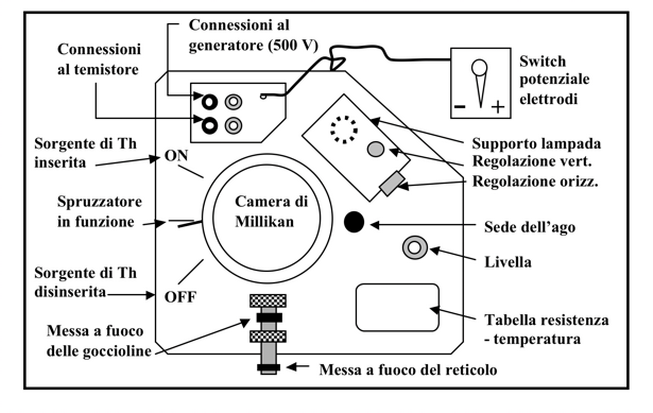
\includegraphics[width=0.9\linewidth]{../images/camera.png}
            \caption{Camera di Millikan}
            \label{fig:camera_millikan}
        \end{figure}
        
        Le misure sono state effettuate ogni volta che si iniziava un nuovo set (ovvero per ogni goccia).
        In tabella \ref{eta} sono riportati i dati relativi a $\eta$ raccolti durante il corso dell'intera sessione di laboratorio: \\
        \begin{table}[H]
        \centering
            \begin{tabular}{ cccc } 
                \toprule 
                orario & R [M$\Omega$] & T [$^o$C] & $\eta$ [Ns/m] \\
                \midrule 
                15:13 &	2,214	&	21,30	&	1,8300E-05  \\
                16:01 &	2,180	&	21,83	&	1,8325E-05  \\	
                16:15 &	2,175	&	21,91	&	1,8329E-05	\\
                16:22 &	2,172	&	21,95	&	1,8331E-05	\\
                16:30 & 2,170	&	21,98	&	1,8331E-05	\\
                17:20 &	2,168	&	22,02	&	1,8333E-05	\\
                17:30 & 2,160	&   22,15	&	1,8334E-05	\\
                17:40 &	2,155	&	22,24	&	1,8345E-05	\\
                17:45 &	2,155	&	22,24	&	1,8345E-05	\\
                18:10 &	2,145	&	22,41	&	1,8353E-05	\\
                \bottomrule           
            \end{tabular}
            \caption{Valori di resistenza e $\eta$ nel corso della durata dell'esperimento}
            \label{eta}
        \end{table}
        Tutti i tempi sono stati misurati con il cronometro di un telefono con risoluzione $0.01$s, di molto più preciso di quanto permettesse la procedura. Si è deciso di arrotondare i tempi alla prima cifra decimale.

\subsection{Misure}
    E' stata misurata la velocità teoricamente uniforme di alcune goccioline d’olio elettricamente cariche, inizialmente in un regime di sola attrazione gravitazionale e in seguito in presenza di un campo elettrico, di intensità nota, diretto lungo la verticale prima in un verso (concorde all'accelerazione di gravità) e poi nell'altro. \\
    Le gocce sono state lasciate cadere nella camera con presa d'aria aperta per favorirne la caduta, dopodiché si è chiusa la camera ed è stato attivato il generatore di differenza di potenziale in direzione opposta a quella della gravità in modo da avere una prima scrematura dalle gocce non cariche. Dopo qualche minuto di attesa è stata ottenuta la condizione cercata e sono iniziate le misure. \\
    Si è deciso di procedere selezionando una goccia, verificare se fosse effettivamente carica immergendola nel campo elettrico, osservarla prima in assenza di campo e solo infine di effettuare le misure con campo elettrico perché spesso si sono osservati moti convettivi non trascurabili che invalidavano la misura. Si è così preso il tempo di caduta sotto effetto della sola gravità per $0.5$mm, prendendo i tempi ogni $0.1$mm e mediandoli. E' stato infatti osservato che i tempi erano più che variabili (per la presenza delle altre gocce cariche e dei pur limitati moti convettivi) e che osservare la caduta di $2.5$mm richiedeva più tempo di quello disponibile e aumentava l'influenza dei moti convettivi sulla caduta. Per le misure in regime di campo elettrico, poichè le gocce cariche si muovevano ad una velocità molto più elevata, sono stati presi i tempi di attraversamento ogni $0.5$mm, 5 volte per ogni configurazione di campo (verso l'alto e verso il basso).
    Sono state quindi trovate per ogni goccia 5 misure di tempi in assenza di campo, 5 con campo rivolto verso il basso e 5 verso l'alto. Spesso si è considerato più opportuno non prendere i tempi continuativamente ma dividendo il moto, così da poter eliminare quei tratti a bassa visibilità o in cui erano concentrate molte gocce che deviavano la traiettoria.\\
    In tabella \ref{gocce} sono riportati per ogni goccia osservata i tempi di caduta in assenza $t$, e in presenza $t_c$ di campo concorde con la forza di gravità; i tempi di salita $t_s$ in presenza di campo opposto alla forza peso; le velocità medie nelle tre configurazioni, rispettivamente $v$, $v_c$, $v_s$ la carica presente su ogni goccia mentre saliva $Q_s$ e scendeva $Q_c$; il raggio della goccia $r$; la distanza tra gli elettrodi $d$; la differenza di densità $\rho$; la distanza $\Delta z$ percorsa dalle gocce per ogni tempo preso in presenza di campo (per la caduta libera $\Delta z = 0.1$mm)

   
\section{Analisi Dati}
    Da ogni set di misure, ovvero per ogni goccia, la prima elaborazione ha riguardato le 5 misure in assenza di campo. Sono stati utilizzati due approci differenti: dai tempi ottenuti è stato calcolato un tempo medio e da questo un raggio per le cinque misure; per ogni tempo è stato calcolato un raggio e dai 5 raggi si è trovato un raggio medio da usare per le seguenti valutazioni. Questo secondo approcio è parso più opportuno in quanto minimizzante gli errori e poiché le risultanti misure erano più coerenti. La relazione utilizzata in questo caso è:
    \begin{equation}\label{raggio}
        r_0 = \sqrt{(\frac{b}{2p})^2+\frac{9\eta v_r}{2g(\rho_{olio}-\rho_{aria})}}-\frac{b}{2p}
    \end{equation}

    Dove $b$ è una costante di correzione per il coefficiente di viscosità, $p$ è la pressione(atmosferica standard), $\rho_{olio}$ e $\rho_{aria}$ sono le densità dell'olio e dell'aria e $v_r$ è la velocità di sedimentazione delle goccioline.\\
    
    
    Per quanto riguarda le misurazioni fatte in presenza di campo è stato osservato che le gocce acquistavano e perdevano carica nel corso della discesa (o della salita ovviamente). Utilizzando il raggio trovato dalla formula \ref{raggio}, per ogni tempo misurato in presenza di campo è stata trovata una carica associata dalla relazione:
        \begin{align}\label{formula carica}
            q = -\frac{4}{3}\pi r^3(\rho_{olio}-\rho_{aria})\frac{g}{E}(1-\frac{V_E}{v_r}) \qq{per goccia che scende} \\
            q = -\frac{4}{3}\pi r^3(\rho_{olio}-\rho_{aria})\frac{g}{E}(1+ \frac{|V_E|}{v_r}) \qq{per goccia che sale}
        \end{align}
    Dove $g$ è la costante di accelerazione gravitazione ed $E$ il campo elettrico generato dalle armature del condensatore.\\
    
    Avendo a disposizione 10 misure di carica per ogni goccia e osservato 10 gocce, sono stati inizialmente considerati 100 valori. Questi sono stati inseriti nella funzione
        \begin{equation}\label{S(q)}
            S(q) = \sum (\frac{Q_i}{k(q)}-q)^2 \quad  \quad k(q) = \lfloor \frac{Q_i}{q} +0.5 \rfloor 
        \end{equation} 
        
    che è stata implementata con un algoritmo che ne restituiva il grafico. La variabile libera $q$ è stata fatta variare intorno ai valori più piccoli ottenuti nel corso delle misure, supponendo che queste potessero essere candidati cariche elementati.

    \begin{figure}[H]\label{Histo:100 data}
    \centering
        \subfloat[\centering S(q) con tutto il set di dati]{{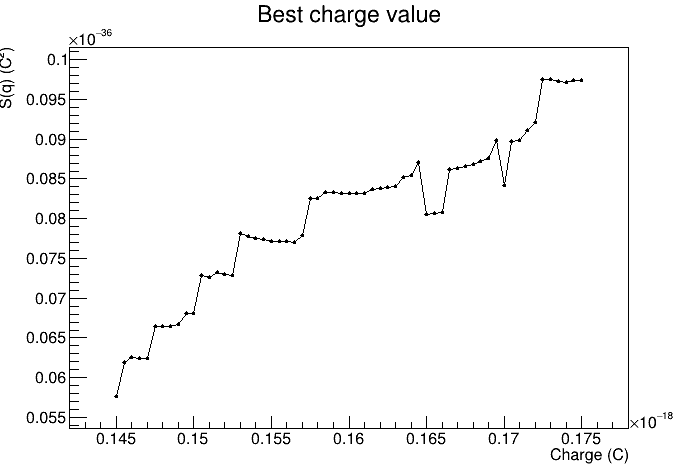
\includegraphics[width=7cm]{../images/Least_Deviation_Squared.png} }}%
        \qquad 
        \subfloat[\centering Istogramma]{{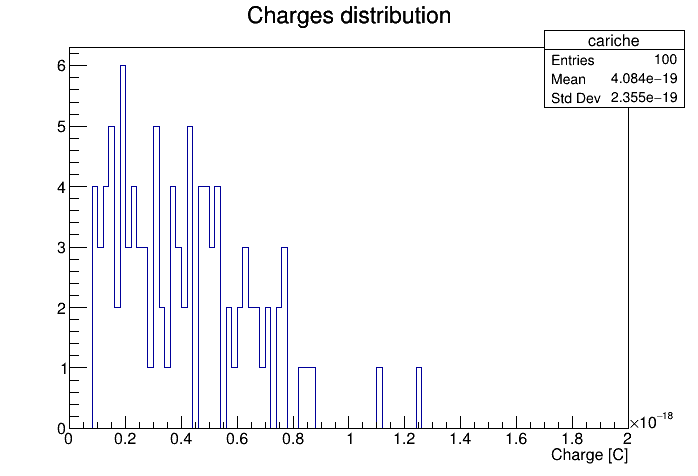
\includegraphics[width=7cm]{../images/100_distribution.png} }}%
        
    \end{figure}
    
    La funzione presentava diversi punti di discontinuità che rendevano pressoché impossibile la visualizzazione di un minimo.
    
    L'algoritmo è stato quindi modificato in modo da scartare per ogni punto di discontinuità le misure che davano mantissa di $K(\qq*{q=q di discontinuità}$$)=0.5$ e valori vicini.
    
    \begin{figure}[H]
    \centering
        \subfloat[\centering S(q) con il set di dati ripulito]{{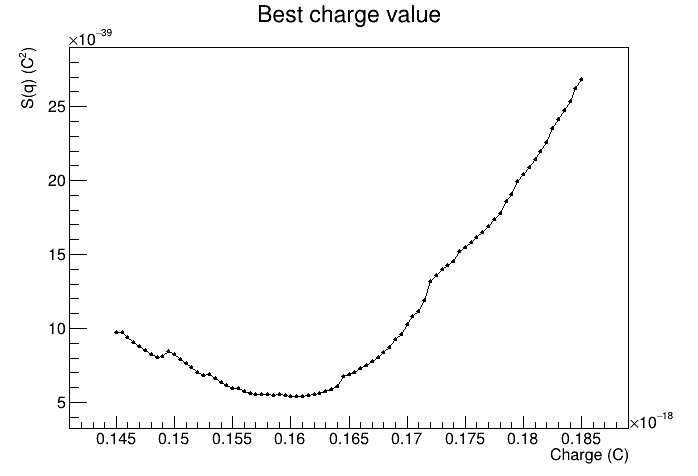
\includegraphics[width=7cm]{../images/best_charges_value.png} }}%
        \qquad
        \subfloat[\centering Istogramma]{{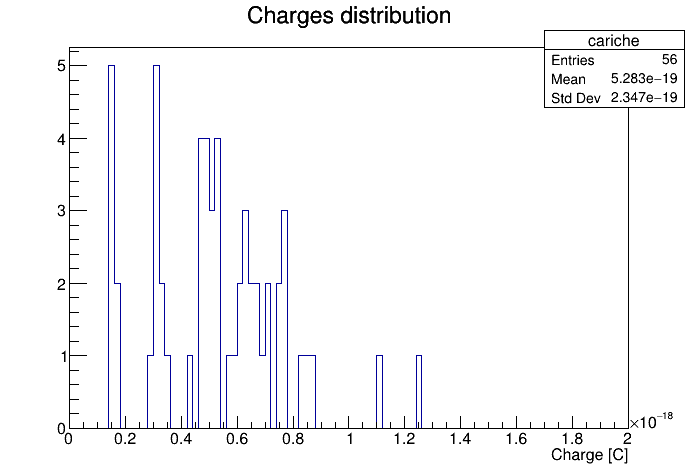
\includegraphics[width=7cm]{../images/Charge_distribution.png} }}%
    \end{figure}

    
    In questo modo il grafico è risultato compatibile con la ricerca del minimo, che è stato valutato dall'algoritmo stesso (che utilizza le librerie di ROOT):
        \[ q_{min} = 1.605 \qq{C}\]
    Intorno a questo valore, K(q) è costante al primo ordine e può essere utilizzato per calcolare la carica elementare:
        \[q_e = \frac{1}{N}\sum_{i=1}^N\frac{Q_i}{k_i(q_{min})}\]
    La miglior valutazione dell'errore è la deviazione standard:
        \[\sigma_{q_e} = \sqrt{\frac{S(q_{min})}{N(N-1)}}\]
    e il valore finale ottenuto è:
          \[ e_{best} = (1.605 \pm 0.013)\cdot 10^{-19} \qq{C}
    \]
    Si è deciso di tenere due cifre significative per l'incertezza poichè $5\cdot10^{-22}$ rappresenta all'incirca $\sim 38,5\%$ di $13\cdot10^{-22}$, il che vuol dire che non è una quantità trascurabile.


\section{Considerazioni finali}
    La valutazione degli errori sistematici risulta essere particolarmente complessa data la variegata natura che questi possono avere tuttavia delle osservaioni possono essere fatte con parziale certezza. Innanzitutto è da subito parso evidente che il moto delle gocce non fosse rettilineo uniforme quando non immerse nel campo elettrico. In questo caso la principale fonte di perturbazione sono stati i moti convettivi che, seppur limitati, non sono stati del tutto eliminati. Spesso le misure sono state interrotte perché la goccia si muoveva verso l'alto o in direzione diagonale. In ogni caso i tempi di percorrenza della stessa goccia di $0.1$mm sono stati di molto diversi. Si ritiene che buona parte delle fonti di errore si siano presentate in questa fase. Il risultato è stato una distribuzione quasi continua di dati, che solo dopo una grossa scrematura sono risultati analizzabili. Un fenomeno che si è pensato potesse influire nella misura è l'attrazione o la repulsione reciproca delle gocce cariche, della quale si è provato a stimare l'ordine di grandezza, considerando gocce sferiche con raggio $10^-6$, carica $10\cdot q$, a distanza $10^-4$:
            \[F_C = \frac{1}{4\pi\epsilon_0}\frac{100q^2}{r^2} \approx 2.3 \cdot 10^{-18} \quad N\]
    Gli effetti sono quindi stati considerati trascurabili rispetto alla forza peso agente sulla stessa goccia d'olio di densità $\rho_{olio} = 860 \frac{kg}{m^3}$:
    \[F_g = \frac{4\pi r^3}{3}\rho_{olio}g \approx 10^{-14}\quad N\]
    , in quanto servirebbero almeno un un centinaio di gocce per avere un effetto significativo.
    Il fatto che le gocce sembrassero perdere e acquistare carica, cosa che può essere spiegato tramite molteplici fenomeni, è sicuramente stato fonte di errore. Si è provato a limitarne gli effetti considerando ogni separata ogni misura, se però nell'arco di tempo della singola misura ($1-3$s c.ca) ci sono stati cambiamenti questo può aver influito nel rendere continua quella che sarebbe dovuta essere una distribuzione discreta. \\
    Una volta isolato il valore finale, è stato fatto un grafico degli scarti quadratici con tutte le misure, è verificabile ad occhio la larghezza delle parabile centrate sui multipli di $q_f$. E' interessante però vedere come sono distrubuite le quantità discrete di carica elementare tra le misure.

    \begin{figure}[H]
        \centering
        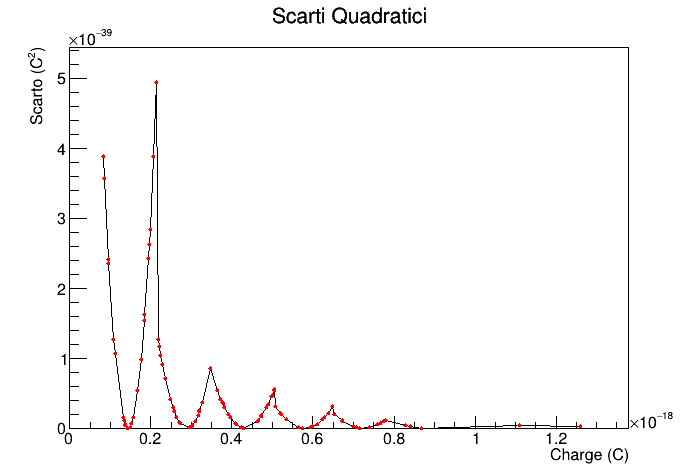
\includegraphics[width=0.7\linewidth]{../images/Scarti.png}
        \caption{Scarti quadratici medi}
    \end{figure}
    
    \subfile{table.tex}
    
\end{document}


